\documentclass[a4paper]{article}
\usepackage[a4paper,left=2.5cm,right=3.5cm,top=2cm,bottom=2cm]{geometry}
\usepackage[utf8]{inputenc}
\usepackage[T1]{fontenc}
\usepackage{csquotes}
\usepackage[style=numeric]{biblatex}
\addbibresource{references.bib}
\usepackage[ngerman]{babel}
\usepackage{graphicx}
\usepackage{tabularx}
\usepackage{mathptmx}
\usepackage{listings}
\usepackage{chngcntr}
\counterwithin{figure}{section}
\usepackage[onehalfspacing]{setspace}

\renewcommand{\refname}{Literaturverzeichnis}
\renewcommand*\contentsname{Inhaltsverzeichnis}

% Dokument
\begin{document}
\parindent0.1cm 

% Titelblatt
\thispagestyle{empty}

\begin{tabular}{ll}
    Name der Schule:& Freies Gymnasium Borsdorf \\
    Fachbereich:& Informatik \\
    Betreuer:& Herr Sauer \\
    Anschrift:& 
    \begin{tabular}{l}
        Heinrich-Heine-Str. 33 \\
        04451 Borsdorf \\
        Deutschland \\
    \end{tabular}
\end{tabular}

\vfill

\begin{center}
    \begin{Huge}
    \textbf{Facharbeit Informatik: \\ \vspace{0.8cm}
    Das Social-Media-Verhalten \\ \vspace{0.8cm}
    von Jugendlichen}\vspace{2cm}
    \end{Huge}
\end{center}

\vfill

\begin{tabular}{ll}
    Verfasser:& Karl Otto Zschiebsch \\
    Anschrift:& 
    \begin{tabular}{l}
        Dorfstraße 11 \\ 
        04828 Plagwitz \\
        Deutschland \\
    \end{tabular}
\end{tabular}

% Inhaltsverzeichnis
\tableofcontents
\doublespacing
\section{Einleitung}

\subsection{Gendergerechte Sprache}

Aus Gründen der besseren Lesbarkeit wird auf die gleichzeitige Verwendung der Sprachformen männlich, weiblich und divers (m/w/d) 
verzichtet. Sämtliche Personenbezeichnungen gelten gleichermaßen für alle Geschlechter. 

\subsection{Motivation}

Die sozialen Medien haben sich seit den letzten 10 Jahren rasant verbreitet. Technologien entwickelt sich immer schneller. Besonders im Bereich der Kommunikation
hat sich dort in den letzten Jahren viel getan. Nach der Entwicklung von E-Mails im Jahre 1971
\footnotemark\footnotetext{\Cite{Kroker14.September.2020}, Michael Kroker: Die Evolution von Social Media: Von der ersten E-Mail 
1971 bis 4 Milliarden Nutzer} kamen weitere Meilensteine wie Listserv 1986 und Facebook im Jahre 2004 hinzu. \newline
Doch die große Revolution sozialer Netzwerke, beginnend 2009 mit WhatsApp, ist heute nicht mehr aufzuhalten. Aus dem Alltagsleben kaum noch 
herauszudenken prägen sie sowohl die 
geschäftliche als auch die private Welt. Schon längst sind aktuelle Beispiele wie der Hype der Gamestop Aktie \footnotemark\footnotetext{\Cite{Diedrich23.06.2021}, Sören Diedrich: Gamestop verdient über eine Milliarde Dollar dank Reddit-Hype 
um eigene Aktie}, entstanden durch die 
sozialen Netzwerk,  mehr Norm als noch Einzelfall. Doch wie wirkt sich all das auf die Jüngsten, auf die Jugendlichen, aus? 
Ist es aufgrund der rasanten Entwicklung in den sozialen Medien möglich, Unterschiede bei nur einem geringen 
Altersunterschied festzustellen? Dies und vieles mehr will ich in meiner Facharbeit herausfinden.

\subsection{Leitfrage und Ziel}

Unter meiner Leitfrage \glqq In wie weit unterscheidet sich die Nutzung von sozialen Netzwerken bei Jugendlichen unterschiedlicher
Altersgruppen?\grqq, will ich vor allem den Konsum und die Nutzung sozialer Netzwerke bei Jugendlichen erfassen 
und Differenzen zwischen den Altersgruppen aufzeigen. Dabei sollen vor allem Daten zur Regelmäßigkeit, Dauer, Gründe und Ziele 
verschiedener Nutzer analysiert werden. Es soll eine Tendenz festgehalten werden, die aufzeigt, wie sich dieser Konsum in den
nächsten Jahren entwickeln vorraussichtlich könnte.
\section{Recherche}

\subsection{Abgrenzung von Begriffen}

Soziale Medien dienen einer häufig profilbasierten Vernetzung und Kommunikation von Benutzern über das Internet  \footnotemark
\footnotetext{\Cite{Bendel}, Oliver Bendel: Soziale Medien}. Nicht als soziale Medien gelten Messenger und Suchmaschinen. Damit 
sind Plattformen wie WhatsApp oder Google unzulässig. Unzulässige Plattformen werden während der Umfrage ignoriert.

Als Jugendliche gelten Personen von 13 bis 18 Jahren. Ergebnisse von Teilnehmern, die zwar die Umfrage ausgefüllt haben, aber nicht
in diese Zielgruppe fallen, wurden tendenziell berücksichtigt, hatten allerdings keine Auswirkungen auf die Umfrageergebnisse.

Die Nutzung einer Plattform definiere ich als vom Nutzer gewollte Interaktion mit der jeweils gewählten Plattform. Schaut die Person zum Beispiel auf einer 
Plattform ein Video, so kann das als gewollte Interaktion und somit als Nutzung bezeichnet werde. Wird allerdings Werbung gesehen,
so ist dies nicht gewollt und zählt somit auch nicht als Nutzung.

\subsection{Verhalten von Jugendlichen in sozialen Medien}

Untersuchungen haben ergeben, dass vor allem die Altersgruppe zwischen 16 und 44 Jahren das Internet
nutzen. Auch nutzen Personen von 10 bis 15 sowie von 45 bis 64 Jahren das Internet sehr regelmäßig \footnotemark\footnotetext
{\Cite{11.August.2020}, Statistisches Bundesamt: Durchschnittliche Nutzung des Internets durch Personen nach Altersgruppen}.
Nach aktuellen Ergebnissen sind YouTube, Facebook, Instagram, Pinterest, Twitch und TikTok die führenden Plattformen in Deutschland
\footnotemark\footnotetext{\Cite{Firsching10.November.2021}, Jan Firsching: Social Media Nutzung in Deutschland 2021: Instagram und 
Facebook dominieren \& YouTube bleibt führende Videoplattform }. Diese Ergebnisse spiegeln nur die Beliebtheit bei deutschen 
Nutzern wider. Ich möchte mit meiner Umfrage  Gemeinsamkeiten und Unterschiede von des Nutzerverhaltens von Jugendlichen 
herausarbeiten. 

Eine Studie von BITKOM zeigte 2011 auf, das 12 \% der Nutzer das Handy für soziale Medien verwenden \footnotemark\footnotetext
{\Cite{Meindl20.Febuar.2012}, Claudia Meindl: Infografik soziale Netzwerke. Mit welchen Geräten der Zugriff erfolgt}. Nach meinen 
subjektiven Beobachtungen halte ich, 10 Jahre nach der Untersuchung, diesen Prozentsatz für nicht mehr realistisch. Hierbei
hoffe ich, aktuellere und zuverlässigere Daten herausarbeiten zu können.

\subsection{Methoden der Datenauswertung}

Mit Hilfe der Umfrage soll eine deskriptive Statistik \footnotemark\footnotetext{\Cite{empirisch}, empirio: So wertest du Ergebnisse 
der quantitativen und qualitativen Forschung richtig aus} erstellt werden. Hierbei werden der Median, der arithmetische Mittelwert,
sowie die Korrelation, also der Zusammenhang, ermittelt. Ich will dabei die qualitative Inhaltsanalyse nach Mayring in fünf Schritten 
vollziehen \footnotemark\footnotetext{\Cite{Pfeiffer06.Dezember.2021}, Franziska Pfeiffer: Qualitative Inhaltsanalyse nach Mayring in 
5 Schritten}. 

Dabei wird zuerst das Material ausgewählt, was in meinem Fall der Umfrage entspricht. 

Danach wird die Richtung der Analyse festgelegt. Hierbei untersuche ich eine Zielgruppe, in meinem Fall Jugendliche am Freiem Gymnasium 
Borsdorf. Ich habe die Zielgruppe deshalb ausgewählt, weil sich diese einfach und effektiv untersuchen lässt.

Im dritten Schritt wird die Form der Inhaltsanalyse gewählt. Hier nutze ich die strukturierende Inhaltsanalyse, welche 
gegebenes Material unter vorher festgelegten Kriterien einschätz. Aufgrund der Umfrage wird diese am besten objektiv 
analysiert.

Im vierten Schritt interpretiere ich die Ergebnisse, indem ich die Antworten für die Auswertung auf einfache Zahlen
reduziere. Dabei werden ausschließlich Ordinalskalen \footnotemark\footnotetext{\Cite{Pfeiffer27.Juni.2018}, Franziska Pfeiffer: 
Fragebogen auswerten mit der Häufigkeitsverteilung in Exel - Vorlage und Tipps} verwendet. Das ist damit begründet, dass in der 
Umfrage keine ja / nein Fragen verwendet werden.

Zum Schluss stelle ich die Gütekriterien sicher. Es wird überprüft, ob die Umfrage
transparent, reproduzierbar und objektiv ist.
\section{Methode}

\subsection{Planung}

Zur Erfassung möglichst vieler Daten habe ich als wissenschaftliche Methode eine Umfrage gewählt. Dab werden zunächst Begriffe 
definiert und abgetrennt, die zu analysierenden Aspekte gesammelt, mögliche Variablen vermerkt und diese auf ihre Messbarkeit geprüft
\footnotemark\footnotetext{\Cite{Konzeption}, Universität Leipzig: Konzeption und Umsetzung}.

Bei der Planung der Umfrage sammelte ich Kriterien, anhand derer man Unterschiede zwischen verschiedenen Altersgruppen erkennen kann.
Der Umfragebogen sollte anfangs nur Online durchzuführen zu sein. Allerdings entschied ich mich dagegen, aufgrund mangelnder Verfügbarkeit
digitaler Geräte in den unteren Klassen.

\subsection{Umfrage}

Innerhalb der Erstellung des Fragebogens überlegte ich mir für jedes Kriterium mehrere passende Fragen. Auf möglich einfache, 
verständliche und eindeutige Fragen wurde geachtet. Dieses überprüfe ich mithilfe einiger Freiwilliger. Dabei bekamen sie eine 
Vorversion des Fragebogens und sollten diesen Ausfüllen. Dadurch konnten zwar Rechtschreibfehler entdeckt werden, allerdings keine 
Probleme in dem Verständnis einzelnen Fragen. Alle daraus gefundenen Fehler wurden korrigiert.

Den Fragebogen erstellte ich sowohl sowohl in Papierform als auch im Onlineformat. Dabei nutzte ich die Plattform Survio.

Die Umfrage wurde von mir auf Datenschutz geprüft und abschließend mit einem entsprechenden Formular an die Schulleitung gesendet.

\subsection{Durchführung}

Nach der Genehmigung des Formulars wurden alle Klassenlehrer kontaktiert. Dabei habe ich nachgefragt, ob ich die Befragung in den
jeweiligen Klassen durchführen kann. Im Falle einer Erlaubnis durch den Klassenlehrer, habe ich  die Anzahl der benötigten 
Umfragebögen ermittelt und diese als auch den Online-Link zur Verfügung gestellt. Die Schüler füllten eigenständig meistens während
einer sozialen Stunde die Umfrage aus. Alle Onlineergebnisse sowie Umfragebögen wurden 
danach in einem einheitlichen digitalen Speicher übertragen.
\section{Auswertung}

\subsection{Dokumentation zur Analyse der Umfragebögen}

Damit ich die Umfrage möglichst einfach und erweiterbar ausfüllen und visualisieren kann, nutze ich die Programmiersprache Java. 
Diese erlaubt mit dem JDK JavaFX, Diagramme zu zeichnen und ermöglicht das Nutzen komplexer mathematischer Formeln.

Zum Abspeichern der Daten nutze ich Java Records, da diese, nach dem sie initialisiert wurden, nicht mehr verändert werden können.
Jede Frage im Umfragebogen wurde kategorisiert. Dabei ergaben sich drei Arten: 

Die erste Art waren Fragen, die dazu dienten, die
Ergebnisse der befragten Person in eine Schublade zu stecken, um so am Ende Unterschiede und Zusammenhänge zwischen einzelnen
Schubläden entdecken zu können. Dazu zählten die Fragen zum Geschlecht und zum Alter. 

Bei der zweiten Art handelte es sich um Fragen,
die die Umfrageteilnehmer selbständig mit individuellen Zahlen ausfüllen sollten. Die hierbei eingegebenen Werte wurden 
paraphrasiert dokumentiert. 

Zum Schluss handelt es sich um ein Multiple Choice Verfahren, indem die Antwortmöglichkeiten vorgegeben waren und der
Befragte nur zutreffendes ankreuzen musste. Jedem möglichen Feld wurde eine Zahl zwischen 0 und 10 zugewiesen. Es wurden alle 
angekreuzten Felder im Record Data dokumentiert.

Die nun folgenden Beispiele sollen dieses veranschaulichen. Sie sind universell gültig, auf ein minimum Reduziert und können auch zum 
Auswerten anderer Umfragen verwendet werden.

Dabei ist NumberHolder ein Record, welches eine reelle Zahl abspeichern kann und QuestionHolder eine Klasse, die ein Array 
zurückgibt, welches die Nummern der Felder aller ausgewählten Fragen beinhaltet.

Alle Fragen wurden nach dem Alter sortiert ausgewertet. Für die Ergebnisse wurden zwei Algorithmen geschrieben, eines für die Fragen
mit individuellen Antworten und eines für Multiple Choice Fragen. Um auf ein vergleichbares Ergebnis trotz schwankender 
Teilnehmeranzahl pro Altersstufe zu kommen, wird alles in Prozent berechnet. Jeder Algorithmus besteht aus zwei Listen, einer 
beinhaltet die totalen Werte und eine die Anzahl an Personen pro Teilnehmer. Die Division ergibt das prozentuale Ergebnis für jede 
Altersgruppe.

Um mit den Algorithmen eine möglichst modulare Struktur zu haben, die sich auf eine Veränderung der Analyse der Fragen anpasst, 
verwende ich Interfaces, welche eine sehr hohe Flexibilität über Lambda-Ausdrücke erreicht.

\subsection{Datenwerte}

Insgesamt wurden 160 Personen am FGB befragt. Von diesen 160 Personen fallen 133 Personen in die zu betrachtende Zielgruppe.
Innerhalb dieser 33 Personen sind 67 Personen männlich, 58 Personen weiblich und 8 divers.

Der Altersduchschnitt aller Befragten liegt bei 15,02 Jahren und innerhalb der Zielgruppe bei 15,34 Jahren. Da das minimale und das
maximale Alter bei jeweils 13 und 18 Jahren liegt, umfasst die Spannweite 6 Jahre und der Median beträgt 15,5 Jahren. Damit liegt 
der Altersdurchschnitt etwas unter dem Median. Dadurch ist das Alter innerhalb der Befragten etwas jünger. 

Die Gesamtteilnehmer nutzen das Internet im Durchschnitt erstmals im Alter von 7,63 Jahren. Bei meiner Zielgruppe liegt die Erstnutzung 
im Alter von 7,68 Jahren. Am Frühesten nutzen Teilnehmer dieses mit 4 Jahren, spätestens mit 12. Der Median und die Spannweite liegen somit bei 8 
Jahren.

In der zweiten Frage liegt die durchschnittliche Nutzung des Internets pro Tag bei allen Befragten bei 4,77 Stunden und innerhalb der 
Zielgruppe bei 5 Stunden. Minimal wurde das Internet 0 Stunden genutzt, maximal 12 Stunden. Der Median liegt damit bei 6 und die 
Spannweite bei 12 Stunden am Tag.

Bei der Frage nach der Regelmäßigkeit gaben von den insgesamt 133 Personen 55 von sich aus an, dass sie das Internet mehr als zwei 
bis dreimal am Tag nutzen. Nur ein Teilnehmer kreuzte an, dass er das Internet seltener als täglich nutzen würde. Niemand gab an, 
dass er seltener als 2 bis 3 mal im Monat das Internet nutzt.

Innerhalb der Befragten war das Handy das mit Abstand beliebteste Gerät zur Nutzung des Internets. Von den insgesamt 133 nutzten 
125 das Handy. Auf Platz zwei lag der Laptop mit 87 Personen. Die am seltensten genutzten Geräte waren jene, die unter Sonstiges
fallen. Dieses Feld wurde von nur 12 Personen angekreuzt.

\begin{figure}[ht]
    \centering
    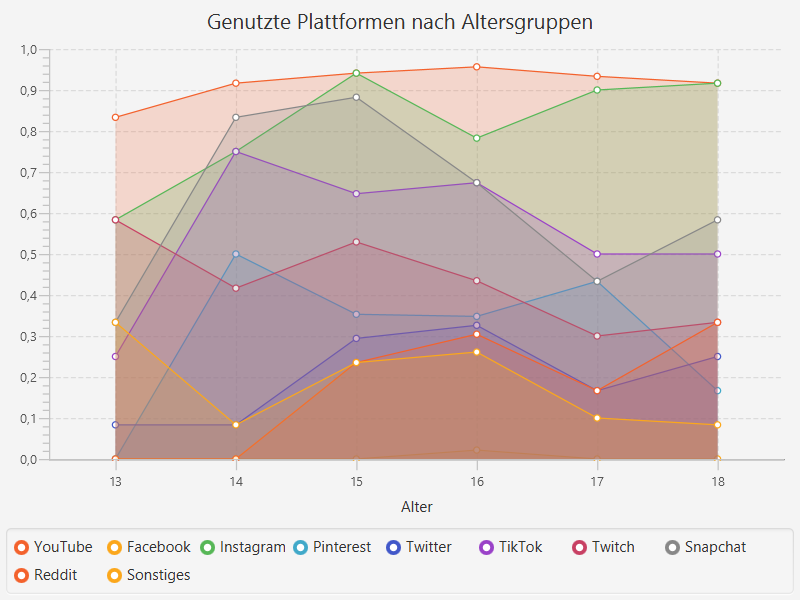
\includegraphics[width=8.5cm]{image/Diagramm Genutzte Plattformen.png}
    \caption{\label{imgs:diagramm_plattformen_datenwerte}Nutzung Social Media basierter Plattformen}
\end{figure}

Als die Umfrageteilnehmer die genutzten Plattformen ankreuzen sollten, lagen YouTube, Instagram, Snapchat und TikTok mit jeweils 120, 106, 80 und 75 Kreuzen 
sehr weit vorne. Sowohl bei der Plattform Pintrest, als auch Reddit konnte ein großer Unterschied zwischen Mädchen und Jungen 
festgestellt werden. Während Pinterest 72,09 \% Frauen nutzen, sind bei Reddit 77,77 \% männliche Nutzer. Facebook lag auf dem letzten
Platz mit einem einzigen Nutzer.

\begin{figure}[h]
    \centering
    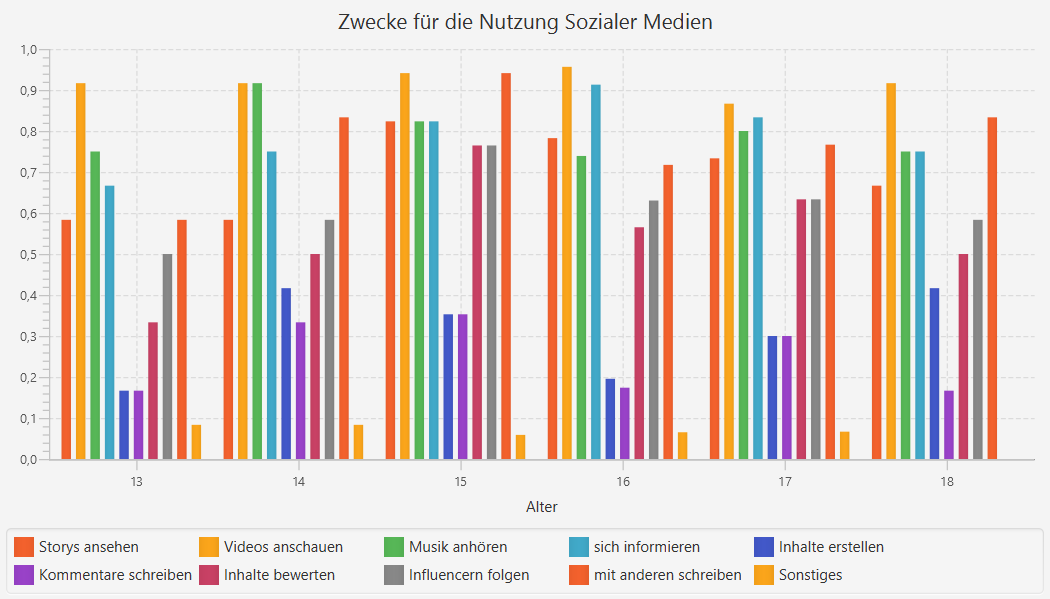
\includegraphics[width=10cm]{image/Diagramm Zwecke der Nutzung.png}
    \caption{\label{imgs:diagramm_zwecke_datenwerte}Zwecke zur Nutzung von sozialen Medien}
\end{figure}

Als Grund für eine Nutzung von sozialen Medien geben 119 Personen an, dass sie unterhalten werden wollen. Es gaben 105 Personen an, 
dass sie sich dort informieren sowie mit Anderen schreiben möchten.

Die Meisten der Befragten nutzen soziale Medien zum Anschauen von Videos (119 Personen), zum Informieren (107 Personen) sowie zum 
Hören von Musik (101 Personen). Besonders selten nutzen die Umfrageteilnehmer soziale Medien zum Erstellen eigener Inhalte 
sowie zum Kommentieren von Inhalten.

In der Frage nach den Gründen sowie nach der Nutzung von sozialen Medien ist das Verhältnis zwischen männlichen und weiblichen Befragten
bei jedem Feld nahezu identisch. Das Verhältnis von Personen mit einer diversen Geschlechteridentität wird bewusst weggelassen, da
diese mit einer Gesamtanzahl von 8 Personen zu niedrig ist, um eine sinnvolle und zielgerichtete Analyse durchzuführen.

\subsection{Regelmäßigkeiten}

\begin{figure}[h]
    \centering
    \includegraphics[width=8.5cm]{image/Diagramm Geräte.png}
    \caption{\label{imgs:diagramm_geraete_regelmaesigkeit}Nutzung von Geräten}
\end{figure}

Das Nutzen von Handys ist durchgängig unabhängig vom Alter auf einem hohen Wert. Dies hängt wahrscheinlich damit zusammen, dass
sie im Vergleich mit anderen Geräten, wie zum Beispiel einem PC, wesentlich günstiger sind sowie den Bonus haben, Verfügbarkeit und
Leistung zu kombinieren.

Einige Plattformen, die zurzeit in der Mode sind, wurden durchgängig unabhängig von der Altersgruppe häufig angekreuzt. Dies war ein 
zu erwartendes Ergebnis, welches lediglich die von den jeweiligen  Plattformen veröffentlichten Nutzerstatistiken bestätigen. Die
einzige Schlussfolgerung daraus ist, dass Jugendliche am FGB im Durchschnitt die selben sozialen Plattformen nutzen wie 
andere Jugendliche auf der ganzen Welt.

Die Plattform YouTube ist die einzige, von den vorgegebenen Plattformen, auf der die Nutzer sich informieren, unterhalten und mit 
anderen schreiben können. Dadurch ergibt sich eine hohe Nutzung, die sehr regelmäßig in allen Altersgruppen ist.

\subsection{Anomalien}

\begin{figure}[h]
    \centering
    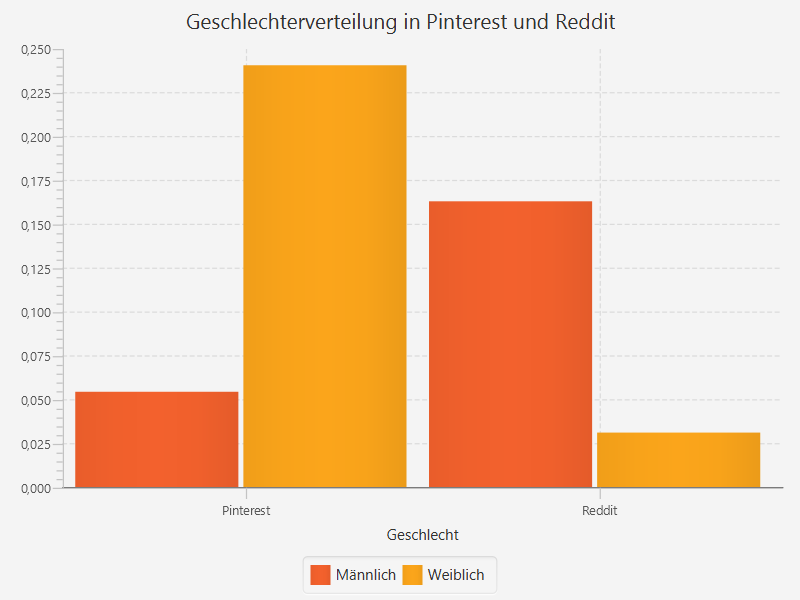
\includegraphics[width=8.5cm]{image/Diagramm Pinterst vs Reddit.png}
    \caption{\label{imgs:diagramm_pinterest_reddit}Geschlechterverteilung bei Pinterest und Reddit}
\end{figure}

Die größte Anomalie bezüglich der Geschlechterverteilung tritt in der Nutzung von Pinterest und Reddit auf. Diese Anomalie konnte 
nicht mit dem Wissen, welches aus anderen Fragen gewonnen wurde, erklärt werden. Ich vermute, dass die angebotenen Inhalte der 
Plattformen diese Diskrepanz hervorrufen.
Da allerdings in der Umfrage nicht nach so etwas gefragt wurde, ist es mir nicht möglich, diese These zu belegen.
Es lässt sich statistisch erkennen, dass die 17-Jährigen die untersuchten Plattformen weniger nutzen. Dieses könnte damit zusammenhängen, dass diese Altersgruppe sich intensiv auf das Abitur vorbereitet und dadurch weniger Zeit für die Nutzung sozialer Medien verwendet.

\subsection{Fehlerbetrachtung}

Die dritte Frage: \glqq Seit wann (Jahr, ungefähr) nutzt du das Internet?\grqq \nobreakspace war ungenau. Diese Frage hätte ich 
besser präzisieren müssen, da im Ergebnis der Befragung ein großer Interpretationsspielraum entstand.
Viele Umfrageteilnehmer füllten diese Frage falsch aus, so dass für die Datenbank die Ergebnisse geändert werden mussten. 
Am Ende musste die Matrix, bestehend aus [JAHR JAHR JAHR JAHR], mit dem Ergebnis übereinstimmen. Beim Paraphrasieren können Fehler
auftreten, wodurch dieser Wert falsch verstanden und somit auch verfälscht eingetragenen wurde.

Die Spannweite vieler Fragen ist vom Median meist sehr weit entfernt. Extremwerte, die hierbei auftreten, hätten allerdings durch die
Masse der befragten Personen ausgeglichen werden sollen. Da ich aber nur 133 Personen, die auch in meiner Zielgruppe fallen, befragt habe,
sind die Mittelwerte der Ergebnisse verfälscht.

Für eine möglichst kleine Fehlerspanne wären daher 500 Befragte 
\footnotemark\footnotetext{\Cite{aussagekraft}, SurveyMonkey: Ab wann ist eine Umfrage aussagekräftig?} notwendig gewesen. Da ich zurzeit 
aber weniger Umfrageteilnehmer habe, rechne ich mit einer Fehlerspanne von etwa 5 \%.
\section{Disskusion}

\subsection{Beantwortung der Leitfrage}

Bei Jugendlichen innerhalb der untersuchten Altersgruppe unterscheidet sich die Nutzung von sozialen Netzwerken kaum. 

Es gibt keine erheblichen Abweichungen in der Beantwortung einzelner Fragen. Festgestellte Anomalien  können nicht vom 
Alter der Person abgeleitet werden. Dies liegt daran, dass
es eine gesamte Altersspanne von nur 6 Jahren gibt. Innerhalb von 6 Jahren sind die Unterschiede hierbei meist nur minimal.

Würde man nun fortlaufend aller 6 Jahre eine solche Umfrage neu durchführen, würde sich im Vergleich zu dieser Umfrage wahrscheinlich 
ein anderes Umfrageergebnisse ergeben. Dies hängt damit zusammen, das nach meiner Analyse meist vorallem die Plattformen genutzt 
werde, die zurzeit in Mode sind. So liegt nach meiner Umfrage Facebook auf dem letzten Platz bei den sozialen Netzwerken, was ein 
komplett anderes Bild ergibt als die Ergebnisse von BITKOM im Jahr 2011.

\subsection{Reflexion}

Ich hätte aufgrund Sars-Cov-19 die Umfrage komplett Online durchführen müssen. Dadurch hätte ich die Möglichkeit gehabt, die Umfrage 
auch dann durchzuführen, wenn Schüler im HomeOffice oder in Quarantäne sind. Zu spät habe ich erkannt, dass mir dadurch ein großer 
Teil meiner Zielgruppe verloren gegangen ist. Daraus resultiert wiederum, dass meine Umfrage weniger repräsentativ ist.

Die Summe der befragten Umfrageteilnehmer ergaben 160 Personen, von denen 133 Personen, 67 männlich, 58 weiblich und 8 diversen 
Geschlechts waren, innerhalb der Zielgruppe fallen. 
Für eine repräsentative Umfrage sind 133 Personen allerdings zu wenig. Um aussagekräftig zu sein, wären
mindestens 500 Personen notwendig gewesen.

Der durchschnittliche finanzielle Status der Eltern eines Schülers am FGB wurde nicht berücksichtigt. Da finanziell besser 
gestellte Eltern ihrem Kind früher ein Gerät kaufen können als Erziehende, bei denen dies nicht so ist, wirkt sich dies auch darauf
aus, ab wann ein Kind erstmals ein solches Geräte nutzen kann. Da am Freien Gymnasium Borsdorf aufgrund des Status als Privatschule 
die Eltern potenziell eher besser verdienen, ist mit einer überdurchschnittlich frühen Nutzung digitaler Geräte zu rechnen. 
Dies stellt allerdings kaum den Durchschnitt der erstmaligen Nutzung dar, weil ausschließlich die Jugendlichen am FGB befragt 
wurden. Um diesen Fakt auszugleichen, hätte man beispielsweise Personen an anderen Schulen befragen können.

Aufgrund der vielen Schulschließungen am FGB hätte ich alle Lehrer schon in den Herbstferien anfragen müssen, um Rechtzeitig alle 
Ergebnisse zu bekommen. Dadurch kam ich in Verzug. Aufgrund einer Sars-CoV-19 Erkrankung musste ich schlussendlich eine
Verlängerung von zwei Wochen beantragen.
\section{Zusammenfassung}

Jugendliche nutzen die sozialen Medien, um unterhalten zu werden, sich zu informieren und um mit anderen zu schreiben. Diese 
Gründe können große Auswirkungen darauf haben, welchen Plattformen beliebt sind und welche nicht. Dies zeigt sich zum Beispiel 
bei der Plattform YouTube.

In der Altersgruppe von 13 bis 18 Jahren sind nach meiner Untersuchung kaum bis keine Unterschiede in Nutzerverhalten festzustellen, 
außgenommen sind die 17 Jährigen aufgrund des Abiturs. Somit kann man auch bei einem geringen Altersunterschied kaum Unterschiede
feststellen.

Erweitert man die Altersspanne der Befragten, würden wahrscheinlich größere Unterschiede sichtbar werden. Dies kann man gut
an der Studie von BITKOM und meiner Umfrage erkennen. Beide Ergebnisse beinhalten die Plattform Facebook. Während in der 
Studie von BITKOM Facebook zu den führenden Plattformen gehört, ist liegt Facebook bei meiner Umfrage auf den letzten Platz.

Im Ergebnis komme ich zu dem Schluss, dass meine Ergebnisse nicht repräsentativ sind. Dies liegt an zu wenigen
Teilnehmern, an einer missverständlich gestellten Frage sowie dem Fakt, das die Umfrageteilnehmer weniger einen durchschnittlichen
Jugendlichen darstellen als vielmehr einen durchschnittlichen Schüler am FGB.
\section{Anhang}

\begin{figure}[h!]
    \centering
    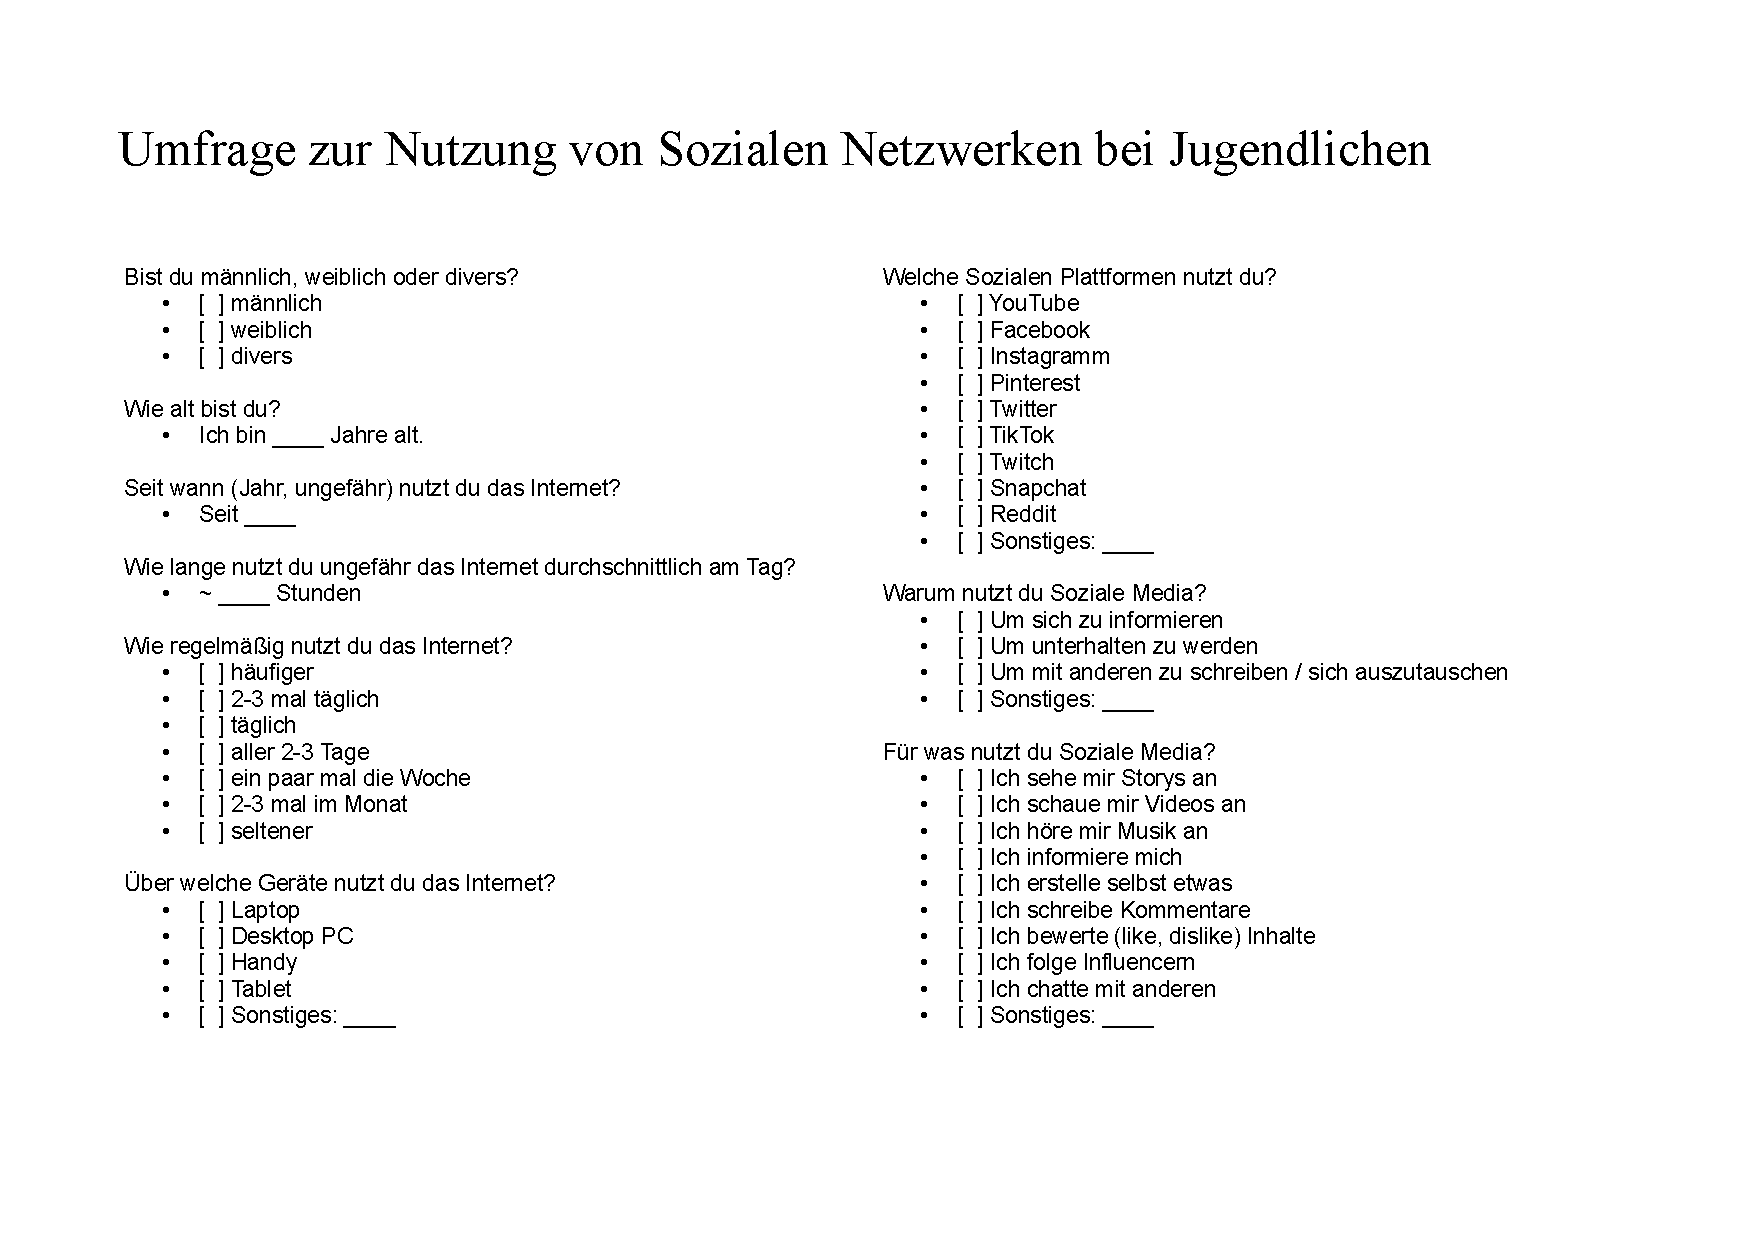
\includegraphics[angle=90, scale=0.7]{image/Umfrage.pdf}
    \caption{\label{imgs:umfrage}Umfrage}
\end{figure}

\begin{figure}[ht]
    \centering
    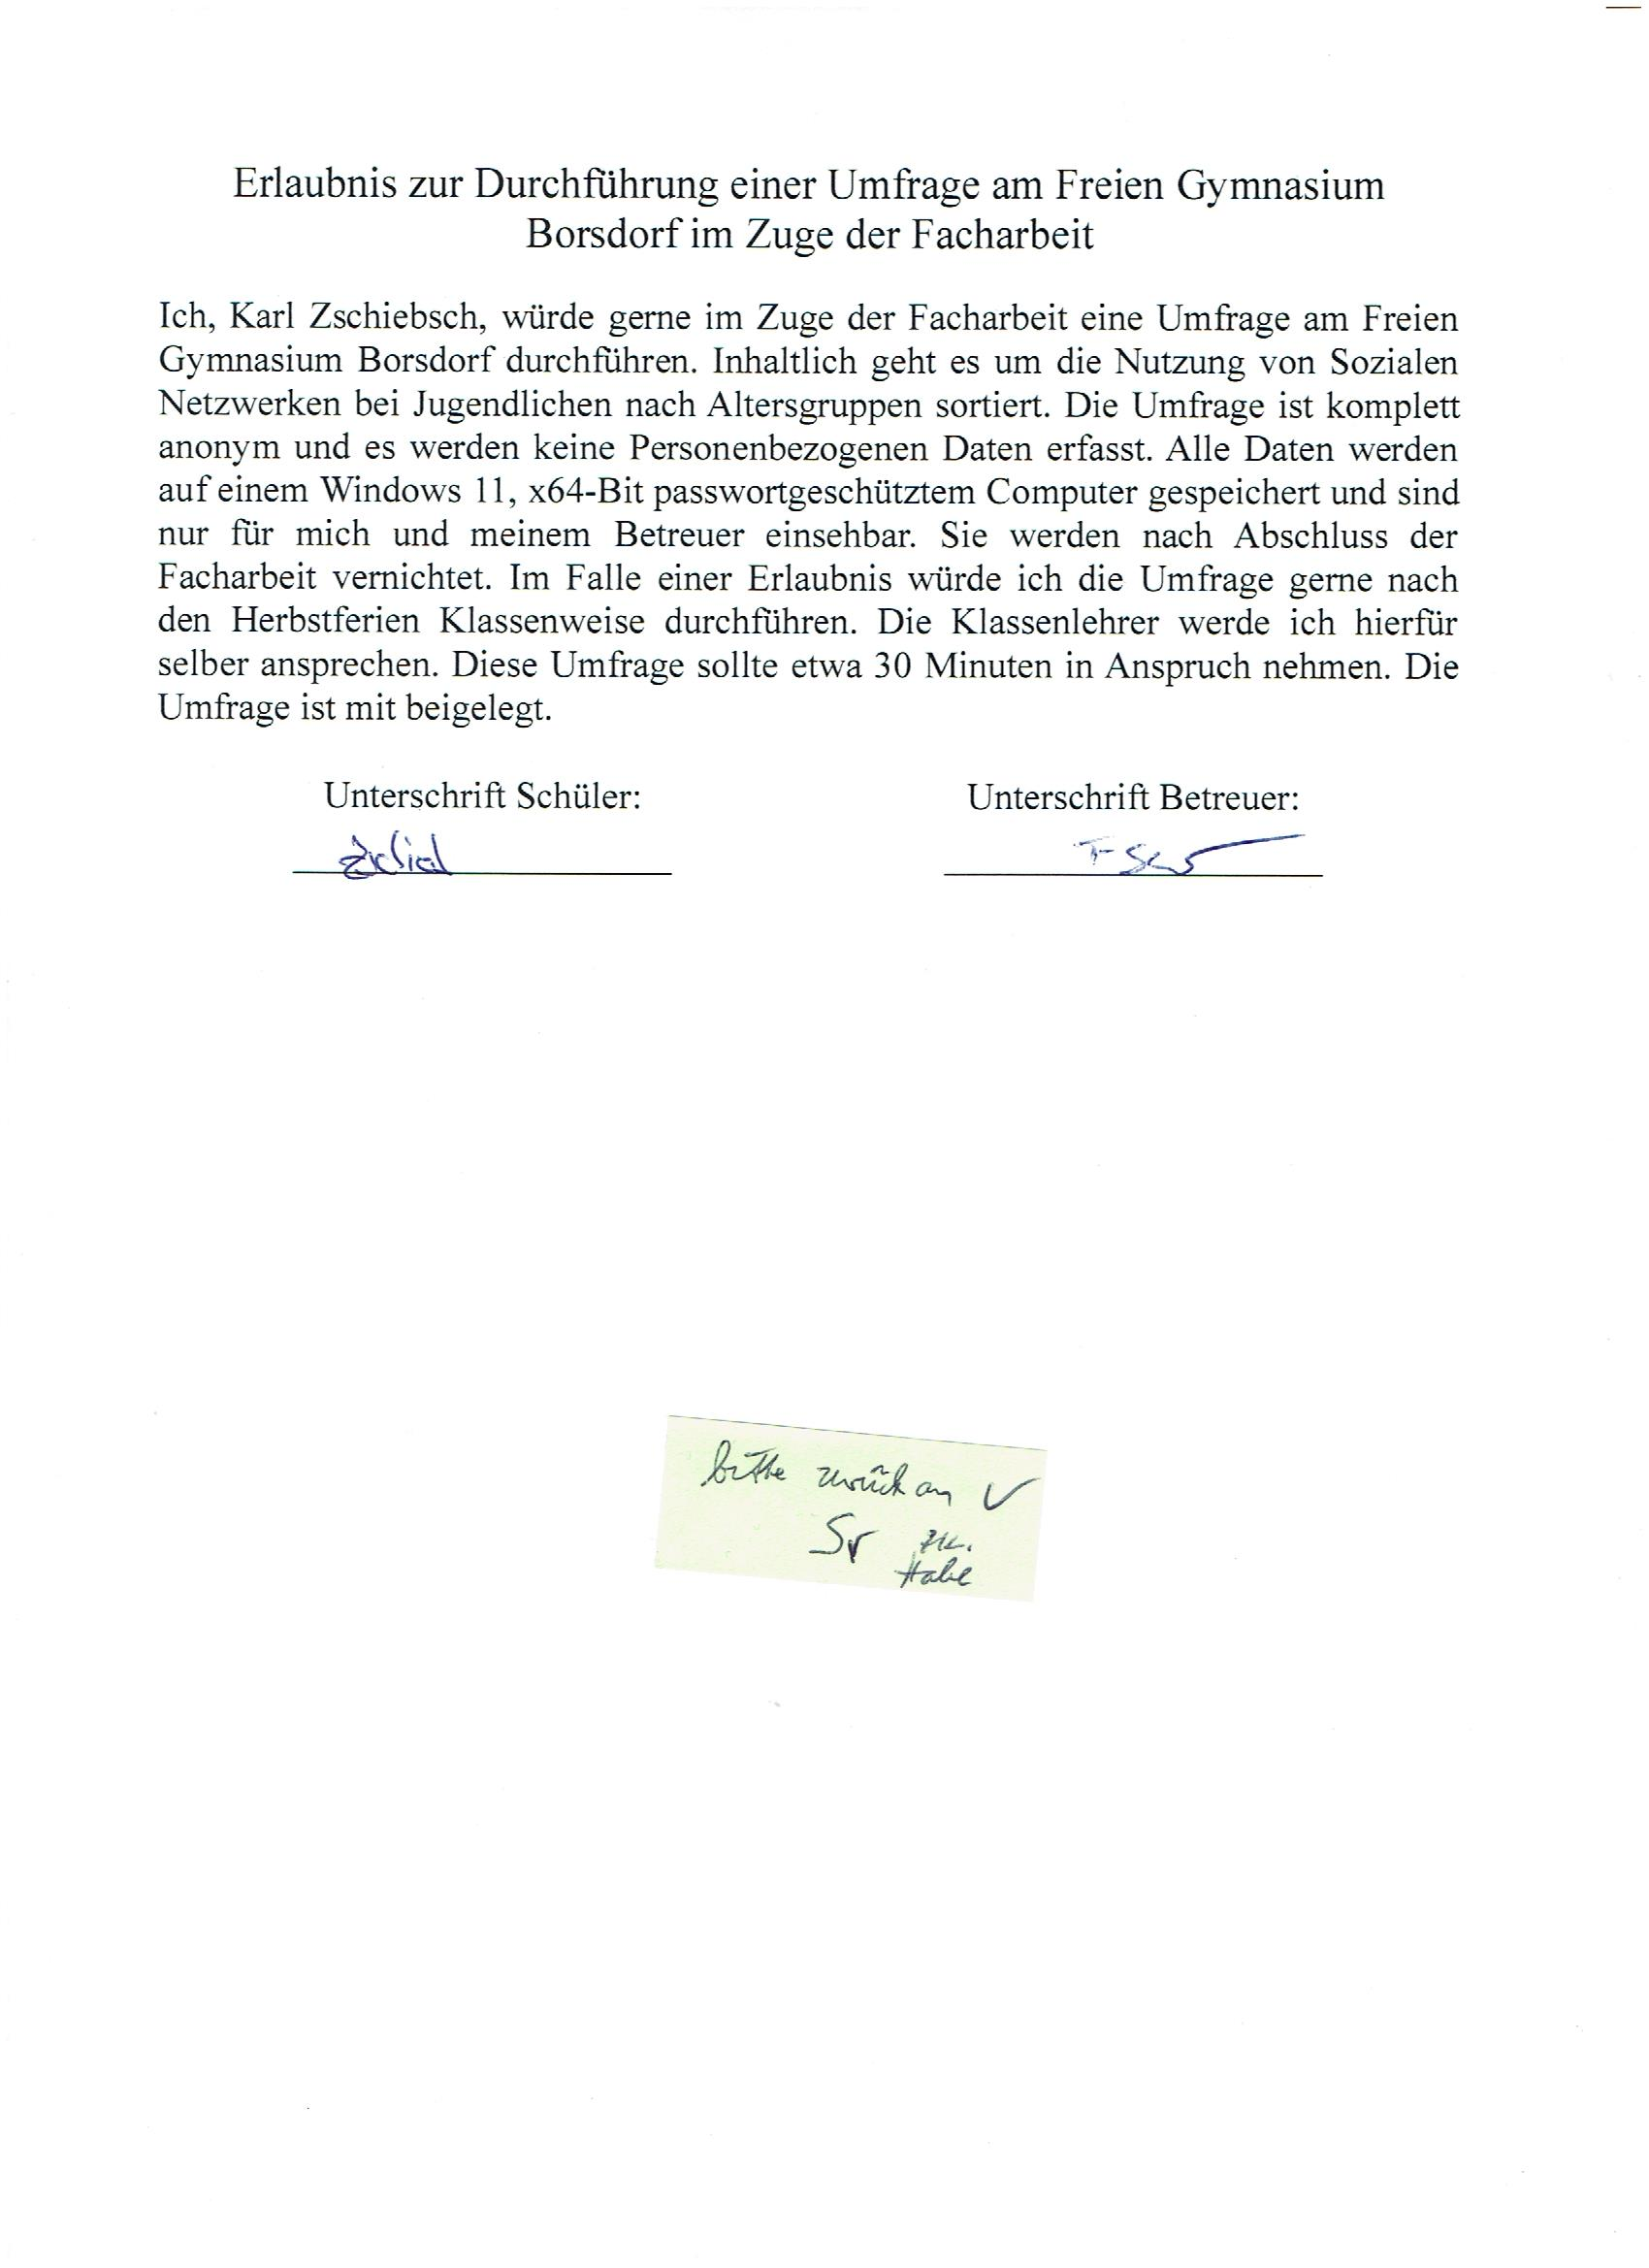
\includegraphics[width=8cm]{image/Genehmigung.jpg}
    \caption{\label{imgs:genehmigung}Genehmigter Antrag auf eine Durchführung der Umfrage}
\end{figure}

\begin{figure}[hb]
    \centering
    \includegraphics[width=8cm]{image/Verlängerung Facharbeit.pdf}
    \caption{\label{imgs:verlaengerung}Genehmigter Antrag auf eine Verlängerung der Facharbeit}
\end{figure}

\begin{figure}[ht]
    \centering
    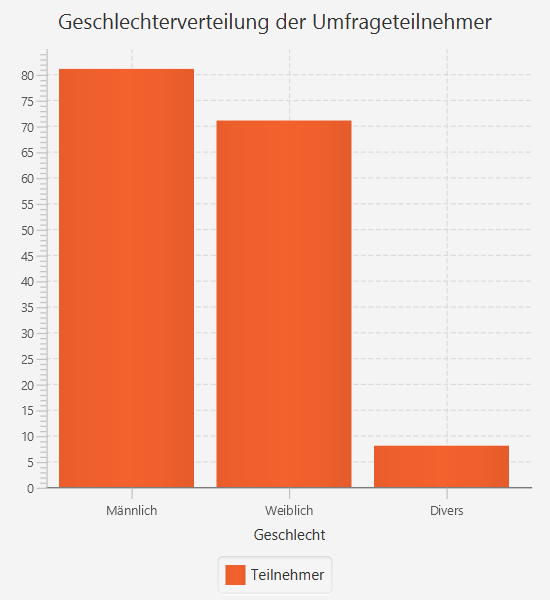
\includegraphics[width=6cm]{image/Diagramm Geschlechterverteilung.png}
    \caption{\label{imgs:diagramm_geschlechter}Geschlechterverteilung der Umfrageteilnehmer}
\end{figure}

\begin{figure}[ht]
    \centering
    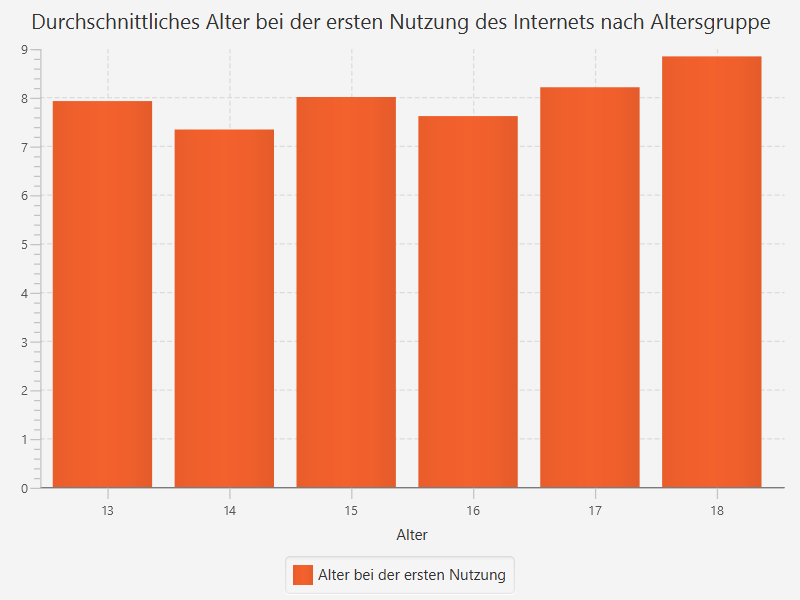
\includegraphics[width=7.25cm]{image/Diagramm Alter bei der ersten Nutzung.png}
    \caption{\label{imgs:diagramm_erste_nutzung}Alter der Umfrageteilnehmer bei der ersten Nutzung des Internets}
\end{figure}

\begin{figure}[ht]
    \centering
    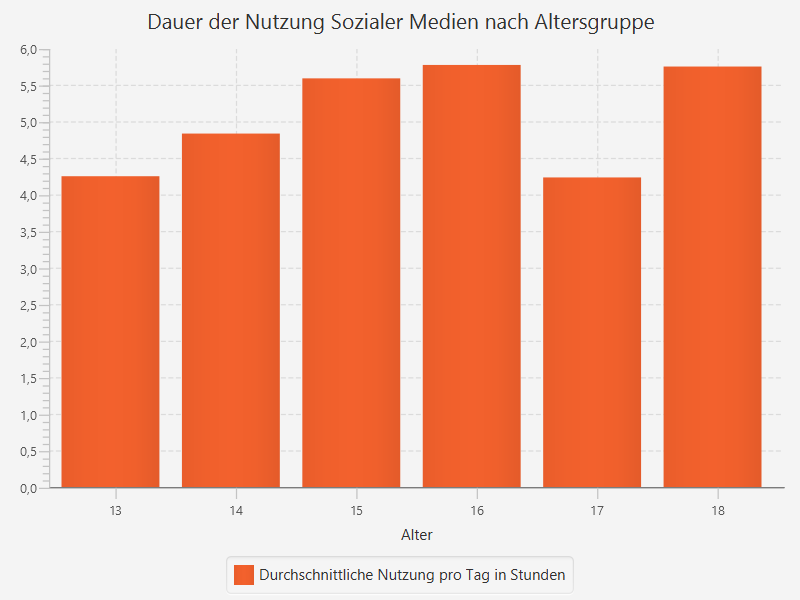
\includegraphics[width=7.25cm]{image/Diagramm Dauer der Nutzung.png}
    \caption{\label{imgs:diagramm_dauer}Dauer der täglichen Nutzung des Internets der Umfrageteilnehmer}
\end{figure}

\begin{figure}[ht]
    \centering
    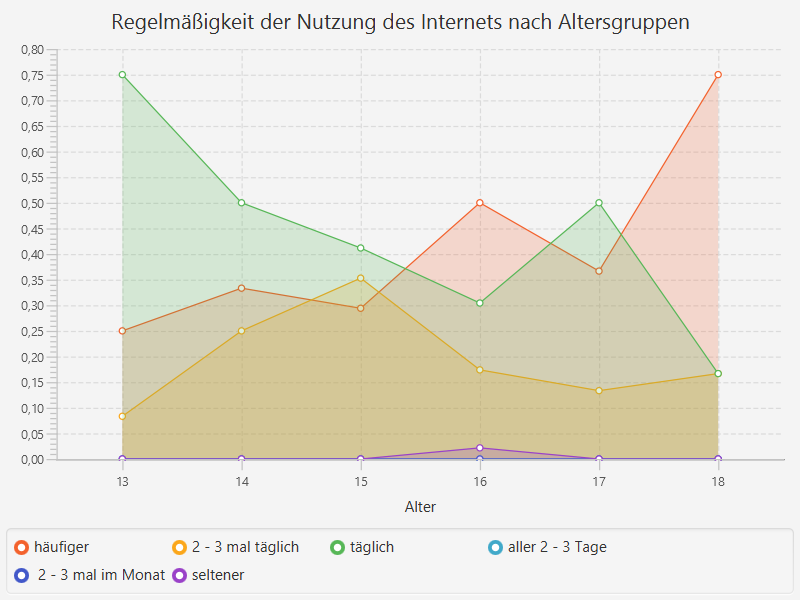
\includegraphics[width=8.5cm]{image/Diagramm Regelmäßigkeit der Nutzung.png}
    \caption{\label{imgs:diagramm_regelmaessigkeit}Regelmäßigkeit Nutzung des Internets der Umfrageteilnehmer}
\end{figure}

\begin{figure}[ht]
    \centering
    \includegraphics[width=8.5cm]{image/Diagramm Geräte.png}
    \caption{\label{imgs:diagramm_geraete}Geräte für die Nutzung des Internets der Umfrageteilnehmer}
\end{figure}

\begin{figure}[ht]
    \centering
    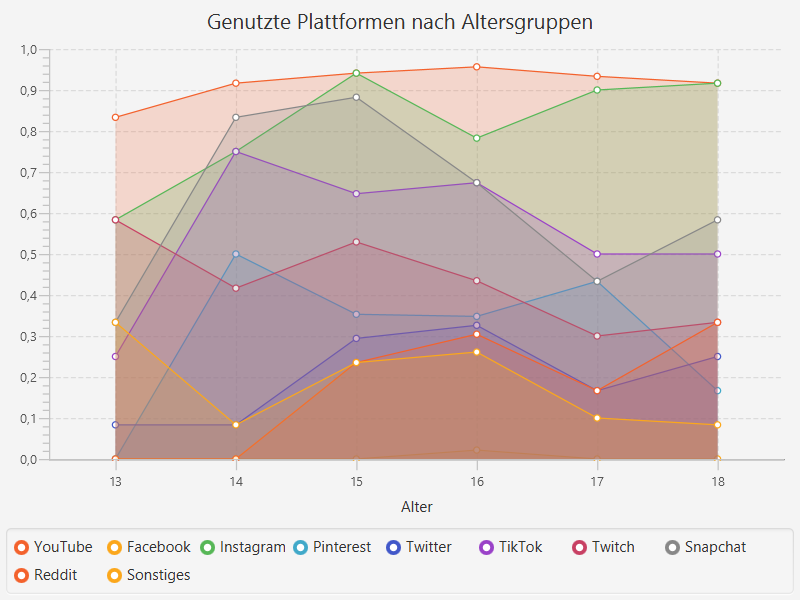
\includegraphics[width=8.5cm]{image/Diagramm Genutzte Plattformen.png}
    \caption{\label{imgs:diagramm_plattformen}Genutzte soziale Netwerke bei den Umfrageteilnehmern}
\end{figure}

\begin{figure}[ht]
    \centering
    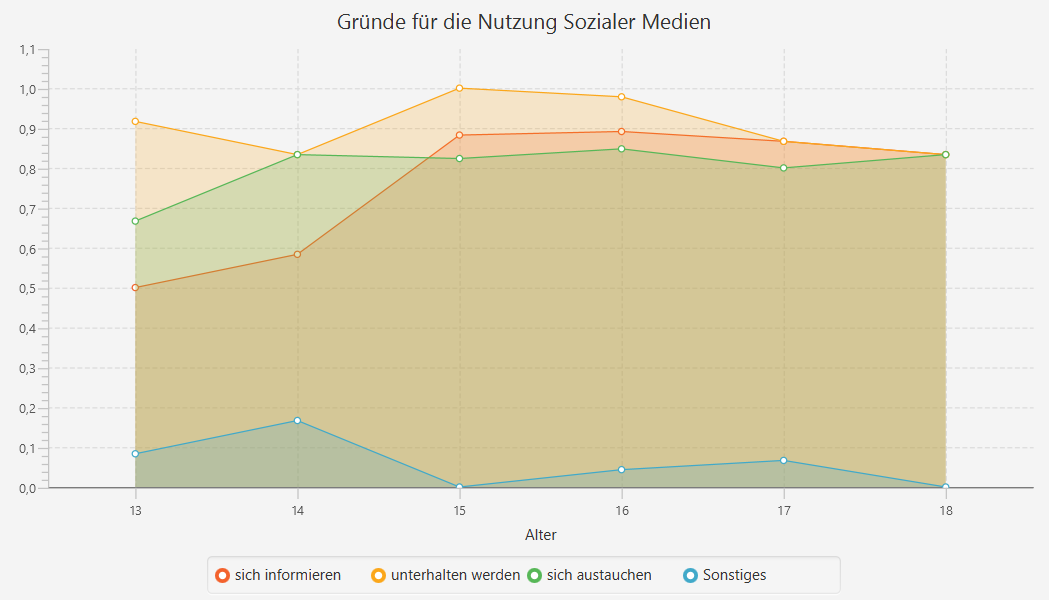
\includegraphics[width=8.5cm]{image/Diagramm Gründe für Soziale Medien.png}
    \caption{\label{imgs:diagramm_gruende}Gründe für die Nutzung sozialer Netwerke bei den Umfrageteilnehmern}
\end{figure}

\begin{figure}[ht]
    \centering
    \includegraphics[width=8.5cm]{image/Diagramm Zwecke für Soziale Medien.png}
    \caption{\label{imgs:diagramm_zwecke}Zwecke für die Nutzung sozialer Netwerke bei den Umfrageteilnehmern}
\end{figure}
\include{chapter/abkürzungsverzeichnis.tex}
\printbibliography[title = {Literaturverzeichnis}, heading=bibnumbered]
\section{Selbstständigkeitserklärung}

Hiermit erkläre ich, \underline{\hspace{5cm}}, dass ich die vorliegende Facharbeit selbst und nur mithilfe 
der vollständig angegebenen Literatur und Quellen im Literaturverzeichnis angefertigt habe.

\vspace{2.5cm}

\begin{tabular}{ll}
    \centering
    \underline{\hspace{6cm}}&\underline{\hspace{6cm}}\\
    (Ort, Datum)&(Unterschrift)\\ 
\end{tabular}


\end{document}